% ==============================================================================
%
%                          O S C I L L O S C O P E
%
% ==============================================================================
\chapter{Oscilloscope} % <<< ------------------------------------------------- %
\label{ch:graphical_front_end}
% ---------------------------------------------------------------------------- %

Because the  FPGA and Linux  side are newly  implemented, and because  the new
transmission protocol  is not the same  as the old one,  existing applications
reading data from the STEMlab no longer function. A new front-end is therefore
required. This front-end is  a web application whose  functionality is broadly
modelled on conventional oscilloscopes; therefore, it is generally referred to
as \emph{scope} in this report. This chapter lays out the requirements for the
scope, explains the design choices on  which it is built, summarizes the major
implementation details, and presents the final product.

% ==============================================================================
%
%                          R E Q U I R E M E N T S
%
% ==============================================================================
\section{Requirements} % <<< ------------------------------------------------- %
\label{sec:gui:requirements}
% ---------------------------------------------------------------------------- %

The requirements  for the scope  are partially  defined by a  Java application
from  previous projects~\cite{gut:specky}  whose core  capabilities are  to be
replicated. More functionality  may be added where  sensible and possible. The
main requirements are:
\begin{itemize}\tightlist
    \item Receive data in configurable size over the network.
    \item Display received data both in the time and fequency domain.
    \item Calculate RMS power density in the signal.
    \item Calculate THD of the signal.
\end{itemize}
% >>>
% ==============================================================================
%
%                         D E S I G N   C H O I C E S
%
% ==============================================================================
\section{Design Choices} % <<< ----------------------------------------------- %
\label{sec:gui:design_choices}
% ---------------------------------------------------------------------------- %

There is  a wealth  of programming  languages to  choose from,  with countless
libraries to go  with them. The following sections explain  why JavaScript and
web technologies are used to implement  the graphical user interface (GUI) and
the mathematical functions of the scope. 

for  this  purpose,  a  group   of  programming  languages  are  compared  and
weighed  against each  other in  various aspects;  the results  are summarized
in   table~\ref{tab:gui:language_choices}.  the   general  attributes   listed
in  table~\ref{tab:gui:language_choices}  are   explained  in  the  subsequent
paragraphs to enable the reader to  understand how they apply to our decision.
Due to its  importance, there is an additional section  dedicated to the topic
of networking (Section~\ref{subsec:gui:networking}).

\paragraph{Open  Standard:} Since this  is a  university project  meant, among
other things, for educational purposes, it  is crucial to make all source code
available to the public under a flexible license. Thus, it is desirable to use
a  technology which  is independent  of any  one company  and their  corporate
policies  (avoiding vendor  lock-in). Some programming  languages are  managed
openly and accept contributions from the public, others not.

\paragraph{Networking:} The  two criteria  which  the data  transfer needs  to
fulfill are  speed and data integrigy.   Since networking is a  highly complex
topic,  it is  important that  the language  not only  has libraries  for good
networking  protocols, but  that those  libraries are  also easy  to use. More
information on the topic is contained in Section~\ref{subsec:gui:networking}.

\paragraph{Graphics:} An oscilloscope is quite a demanding application when it
comes to graphics; drawing an image stream  which looks fluid to the human eye
on modern  high resolution display  uses a  lot of processing  power. Using an
interface such as  OpenGL which can utilize dedicated graphics  resources on a
computer is therefore necessary.

Additionally, creating a  sensible user interface with  basic drawing commands
such as rectangles  and lines is impractical. Instead, a GUI  toolkit to speed
up the design process is needed.

\paragraph{Prevalence:} Using a  technology which is widespread  makes it more
likely that good tutorials are available. It also facilitates troubleshooting,
since a larger  user base means that  there is a higher chance  of savvy users
being able to provide support if needed.

\paragraph{Ease  of  Development:} Some  solutions   require  large  IDEs  and
unwieldy  toolchains  for   development. Others  can  be  used   with  a  more
lightweight  setup. Since both  team  members come  from  a Linux  background,
the  latter  is preferred. Since  added  complexity  always also  means  added
probability  of errors  and failures,  using leaner  tools also  decreases the
chances of having to fight with  the development tools instead of tackling the
actual challenges which are to be solved.

\paragraph{Ease of Deployment:} This takes into  account how easy or difficult
it is for an end-user to install the scope and get it up and running. Having a
toolchain which allows the effortless creation of stable binaries is important
here.

\paragraph{Familiarity With The Language:} The best  toolkits do not matter if
none of  the involved programmers have  ever used them and  will struggle with
even  the basics  for  a major  part  of the  project's  duration. Thus it  is
inevitable that personal preferences also flow into the decision process.

\begin{table}
    \centering
    \caption[Comparison of Programming Languages]{%
        A comparison  of a few  programming languages  which might be  used to
        implement  a  graphical  front-end  like the  oscilloscope  from  this
        project. The scale goes from \num{1} (worst) to \num{6} (best).%
    }
    \label{tab:gui:language_choices}
    \begin{tabular}{lrrrrr}
        \toprule
                                        & \parbox[t]{2mm}{\rotatebox{90}{Rust}}
                                        & \parbox[t]{2mm}{\rotatebox{90}{C++}}
                                        & \parbox[t]{2mm}{\rotatebox{90}{Java}}
                                        & \parbox[t]{2mm}{\rotatebox{90}{Python}}
                                        & \parbox[t]{2mm}{\rotatebox{90}{JavaScript}}\\
        \midrule
        Open Standard                   &  6 &  6 &  1 &  6 &  6 \\
        Networking                      &  6 &  6 &  6 &  6 &  4 \\
        Graphics                        &  2 &  5 &  5 &  5 &  6 \\
        Prevalence                      &  3 &  6 &  6 &  5 &  6 \\
        Ease of Development             &  5 &  5 &  5 &  5 &  6 \\
        Ease of Deployment              &  3 &  4 &  5 &  6 &  6 \\
        Familiarity With the Language   &  3 &  3 &  4 &  6 &  6 \\
        \midrule
        Total                           & 28 & 35 & 32 & 39 & 40 \\
        \bottomrule
    \end{tabular}
\end{table}

\paragraph{Summary:} As          the          total         scores          in
Table~\ref{tab:gui:language_choices} show, JavaScript  fits the priorities set
in this project best. As  a scripting language which can be  run in any modern
browser, a website  can be provided by  the STEMlab board and  accessed from a
client via  a browser. Since no special  programs need to be  installed on the
client  computer, and  every major  operating system  today has  at least  one
reasonably modern  browser, this makes  the solution both highly  portable and
easy to deploy from an end-user perspective.

JavaScript's  popularity ensures  that there  is no  danger of  the underlying
technology  of  the  scope   becoming  obsolete  any  time  soon. Furthermore,
with  its support  for  WebGL and  the WebSockets  protocol,  it provides  two
performant and easy-to-use technologies  to implement graphics and networking,
respectively. Its primary downside is a heavy memory footprint, but since that
is  rarely a  concern on  modern computers,  it is  not considered  a relevant
factor for our decision.

% >>>
% ==============================================================================
%
%                          N E T W O R K I N G
%
% ==============================================================================
\subsection{Networking} % <<< ------------------------------------------------ %
\label{subsec:gui:networking}
% ---------------------------------------------------------------------------- %

For networking, two primary protocols are available: UDP and TCP.  To ensure a
fluid stream of data, minimizing protocol overhead is key. In situations where
data integrity is not essential, UDP is generally used. It carries no overhead
for guaranteeing completeness and correct order of packages.

If data  integrity is vital, TCP  is generally the protocol  of choice. It has
mechanisms  for  guaranteeing  both  the completeness  and  correct  order  of
packages.  This comes at the cost  of some overhead, but in most applications,
this is negligible and well worth the cost. Another key feature of TCP is that
it can perform congestion control. TCP will  sent no more packages if previous
packages  have  gone missing  (i.e. TODO:  if  their  reception has  not  been
confirmed?).  Where UDP will happily flood the network with as much data as it
is fed,  TCP ensures that  the network is not  flooded. The result is  that in
case of a  bad or slow network  connection, the amount of  transmitted data is
automatically adapted  to the network,  and only as much  data is sent  as the
client can actually receive and process.

When  deciding how  to  deploy TCP,  one  can choose  to  implement one's  own
subprotocol,  or  use  one  of   the  existing  two: HTTP  or  WebSockets. The
WebSockets  subprotocol,   being  intended  for  data   streaming  and  having
mature  JavaScript   support,  fits   the  requirements  of   our  application
perfectly.    Some  additional   notes   on  WebSockets   can   be  found   in
Appendix~\ref{sec:app:gui:websockets} on page~\ref{sec:app:gui:websockets}.

%>>>
% ==============================================================================
%
%                              P R O D U C T
%
% ==============================================================================
\section{Product} % <<< ------------------------------------------------------ %
\label{sec:gui:product}
% ---------------------------------------------------------------------------- %

\begin{figure}
    \centering
    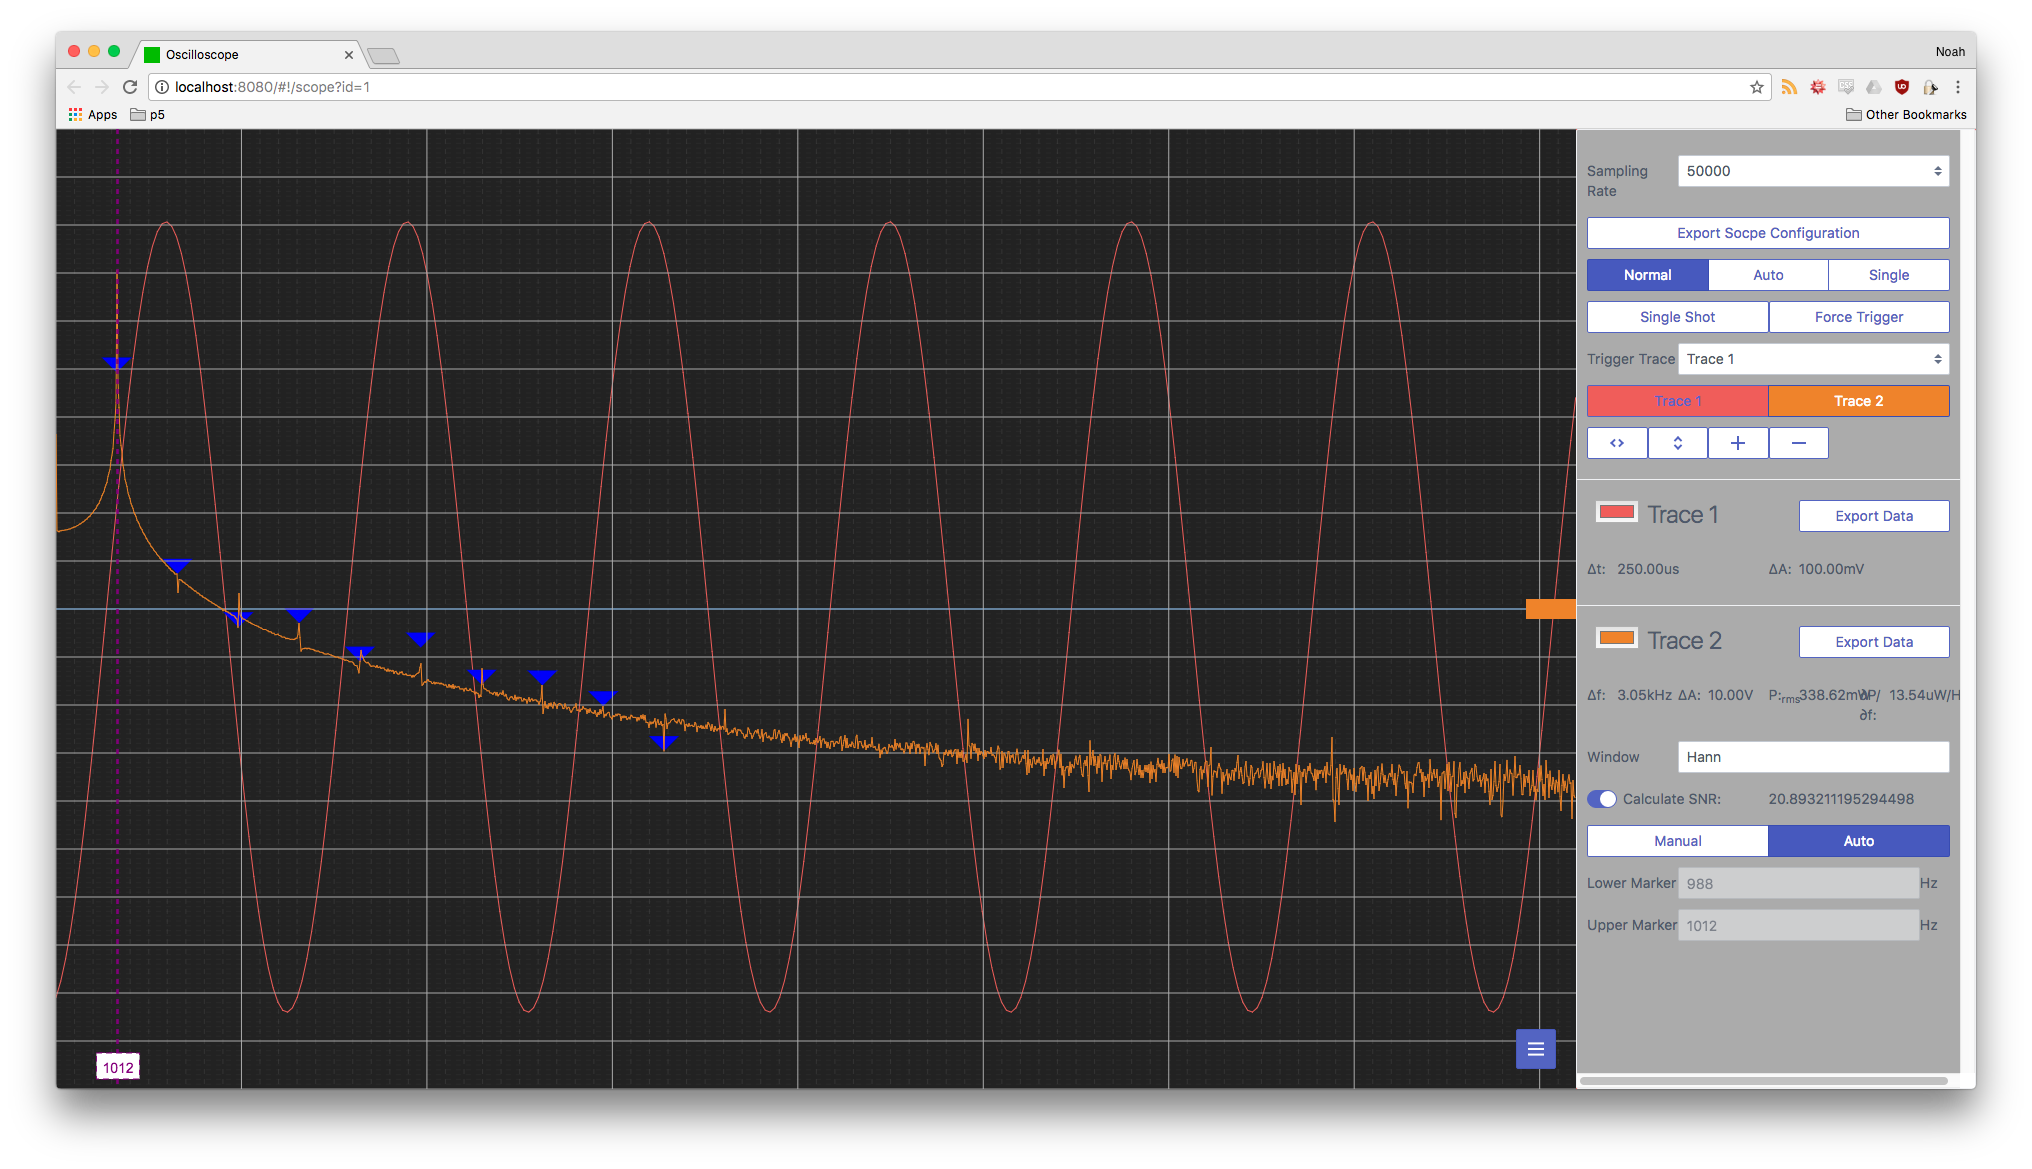
\includegraphics[width=1\textwidth]{images/gui/scope}
    \caption[The scope application]{%
        The scope application in it's current state, displaying time and FFT data.%
    }
    \label{fig:gui:screenshot}
\end{figure}

The oscilloscope  is a web  application that can  be directly loaded  from the
server  running on  the  STEMlab. It  has the  following  capabilities in  its
current implementation:
\begin{itemize}\tightlist
    \item 
        Receive data over  the network for two channels (this  is only limited
        by the physical channels of the STEMlab).
    \item 
        Manage triggering set a trigger type,  level and the number of samples
        that have to be recorded before and after the trigger is activated.
    \item 
        Calculate and display the power density spectrum.
    \item 
        Calculate the SNR both automatically detecting the signal and manually
        being told where the signal is.
    \item 
        Calculate the THD for a given base harmonic. TODO: !
    \item 
        Export data to an array-string.
    \item 
        Export and load the scope configuration to and from JSON strings.
\end{itemize}
The  following  pages  explain  how   the  application  is  structured,  along
with  the  implementation  of  some  of  its  key  features. A  screenshot  in
Figure~\ref{fig:gui:screenshot}  shows the  overall layout  and design  of the
scope.


% ==============================================================================
%
%                  A P P L I C A T I O N   S T R U C T U R E
%
% ==============================================================================
\subsection{Application Structure} % <<< ------------------------------------- %
\label{subsec:gui:application_structure}
% ---------------------------------------------------------------------------- %


The  entire   application  consists  of   a  single  state   tree. This  makes
it   very   easy   to   import    and   export   settings   and   presents   a
better   overview   of   the   application   state   than   scattering   state
information   across  various   objects.   Listing~\ref{lst:gui:app_structure}
in              Appendix~\ref{sec:app:gui:state_tree_of_scope}              on
page~\pageref{sec:app:gui:state_tree_of_scope}   shows  an   extract  of   the
tree   structure. Like   any    JavaScript   application,   the   oscilloscope
runs     asynchronously. Its    eventloop     structure     is    shown     in
Figure~\ref{fig:gui:eventstructure}.

\begin{figure}
    \centering
    \begin{tikzpicture}[%
        align=center,
        text=q1,
        draw=sq5,
    ]
    \small
    \sffamily

    \begin{scope}[
        every node/.style = draw,
        terminal/.append style={
            rounded rectangle,
            fill=sq5,
            text=q1,
            inner sep=2mm,
        }, % data packages
        sign/.style={
            inner sep=2mm,
            rounded corners=1mm,
            fill=sq5,
            text=q1,
        },         % custom signal style
        circ/.style={
            inner sep=2mm,
            rounded corners=1mm,
            double,
            fill=sq5,
            draw=q1,
            text=q1,
        }, % circuitry
        proc/.style={
            inner sep=2mm,
            rounded corners=1mm,
            fill=sq5,
            text=q1,
        },       % process/activity
        dec/.style={
            inner sep=2mm,
            rounded corners=1mm,
            fill=sq5,
            text=q1,
        },       % decision/activity
        stor/.style={
            fill=cyan!30
        },         % storage
        dbtable/.style={
            text=sq5,
            draw=q1,
            rounded corners=1mm,
            inner sep=2mm,
        } % database tables
    ]
        \node (newUART) [
            dec,
            align=center,
            diamond,
            minimum width=33mm,
            minimum height=33mm,
        ] at (0,0) {neuer\\UART\\Request?};
        \node (init) [
            proc,
            above=of newUART,
            align=center,
        ] {Hardware\\initialisieren};
        \node (forMe) [
            dec,
            align=center,
            diamond,
            right=of newUART,
            minimum width=33mm,
            minimum height=33mm,
        ] {F\"ur mich?};
        \node (package) [
            proc,
            right=of forMe,
            align=center,
        ] {Datenpaket mit\\Moving Average\\ und Addresse\\erstellen};
        \node (crc) [
            proc,
            below=of package,
            align=center,
        ] {CRC brechnen\\und zu Daten\\hinzuf\"ugen};
        \node (send) [
            proc,
            left=of crc,
            align=center,
        ] {Datenpaket\\senden};
        \node (getADC) [
            proc,
            below=of send,
            align=center,
        ] {ADC-Messung\\ausf\"uhren};
        \node (movAvg) [
            proc,
            below right=of getADC,
            align=center,
        ] {Moving\\Average\\berechnen};
        \node (LED) [
            proc,
            below left=of movAvg,
            align=center,
        ] {LED\\blinken\\lassen};
        \node (systick) [
            proc,
            above left=of LED,
            align=center,
        ] {auf n\"achsten\\\texttt{systick} warten};
    \end{scope}

    \begin{scope}[
            rounded corners,
            every path/.append style={draw=q1,},
            >=latex',
    ]
        \draw[-latex] (init) -- (newUART);
        \draw[-latex] (newUART) -- node[midway,anchor=south] {ja} (forMe);
        \draw[-latex] (forMe) -- node[midway,anchor=south] {ja} (package);
        \draw[-latex] (package) -- (crc);
        \draw[-latex] (crc) -- (send);
        \draw[-latex] (forMe) edge[bend left] node[midway,anchor=north] {nein} (newUART);
        \draw[-latex] (send) edge[bend left] (newUART);
        \draw (newUART) edge[loop below]  node {nein} (newUART);

        \draw[-latex] (getADC) edge[bend left] (movAvg);
        \draw[-latex] (movAvg) edge[bend left] (LED);
        \draw[-latex] (LED) edge[bend left] (systick);
        \draw[-latex] (systick) edge[bend left] (getADC);

    \end{scope}

\end{tikzpicture}
    \caption[Scope Event Structure]{%
        The scope's event structure
    }
    \label{fig:gui:eventstructure}
\end{figure}

All of the values  that can be controlled through the GUI --  and many more --
are  also controllable  directly through  the state  tree. Upon initialization
of  the  application, the  entire  state  tree  is  loaded and  references  to
parts  of it  are passed  to  the controller  objects.  The  structure of  the
application  is hierarchical;  the most  important relations  are depicted  in
Figure~\ref{fig:gui:structure}.  In  the following some of  the more important
prototypes  and functions  from Figure~\ref{fig:gui:structure}  are elaborated
upon.

\begin{figure}
    \centering
    \tikzsetnextfilename{gui-structure}
\begin{tikzpicture}[%
    %show background grid,
    font=\small,
]
    \begin{class}[text width=4.5cm]{Oscilloscope}{0,0}
        \operation{draw(void)}
    \end{class}
    \begin{class}[text width=4.5cm]{Source}{0,-3}
        \operation{forceTrigger(void)}
        \operation{samplingRate(s: u32)}
        \operation{frameConfiguration(frameSize: u32, pre: u32, suf: u32)}
        \operation{triggerOn(trigger: Trigger)}
        \operation{single(channel: u32)}
        \operation{normal(channel: u32)}
        \operation{auto(channel: u32, timeout: u32)}
    \end{class}
    \begin{class}[text width=4.5cm]{WebSocketSource}{6,-4.15}
        \inherit{Source}
        \operation{sendJSON(string: String)}
        \operation{onOpen(void)}
        \operation{onMessage(e: Event)}
    \end{class}
    \begin{class}[text width=4.5cm]{Trace}{0,-9}
        \operation{draw(canvas: Canvas)}
        \operation{calc(void)}
    \end{class}
    \begin{class}[text width=4.5cm]{TimeTrace}{6,-8.7}
        %\inherit{Trace}
    \end{class}
    \begin{class}[text width=4.5cm]{FFTrace}{6,-10.3}
        %\inherit{Trace}
    \end{class}
    \begin{class}[text width=4.5cm]{GeneralPrefPane}{6,-0.3}
    \end{class}
    \begin{class}[text width=4.5cm]{TimeTracePrefPane}{6,-7.2}
    \end{class}
    \begin{class}[text width=4.5cm]{FFTracePrefPane}{6,-11.8}
    \end{class}
    %\composition{Oscilloscope}{source}{1}{Source}
    \composition{Oscilloscope}{}{}{Source}
    \composition{Source}{}{}{Trace}
    \composition{Oscilloscope}{}{1}{GeneralPrefPane}
    \composition{TimeTrace}{}{}{TimeTracePrefPane}
    \composition{FFTrace}{}{}{FFTracePrefPane}

    \node[text=black,anchor=west] at ($(Oscilloscope.south) - (0,2ex)$) {source};
    \node[text=black,anchor=east] at ($(Source.north) + (0,1.5ex)$) {1};
    \node[text=black,anchor=west] at ($(Source.south) - (0,2ex)$) {traces};
    \node[text=black,anchor=east] at ($(Trace.north) + (0,1.5ex)$) {1..*};
    \node[text=black,anchor=east] at ($(FFTracePrefPane.north) + (0,1.5ex)$) {1};
    \node[text=black,anchor=east] at ($(TimeTracePrefPane.south) - (0,2ex)$) {1};

    \draw [umlcd style inherit line] ($(Trace.east) + (0,1.5mm)$) -| (TimeTrace.south);
    \draw [umlcd style inherit line] ($(Trace.east) - (0,1.5mm)$) -| (FFTrace.north);
\end{tikzpicture}

    \caption[The scope structure]{%
        The structure of the scope application with its major relations%
    }
    \label{fig:gui:structure}
\end{figure}

% ==============================================================================
%
%                                  N O D E S
%
% ==============================================================================

\paragraph{The  \code{Oscilloscope} prototype}  is  the  top level  controller
which contains  exactly one source. It  is responsible for handling  all mouse
events  and  reacting  accordingly,  such  as  moving  the  trigger  level  or
zooming and  panning.  The Oscilloscope  draw call is responsible  for drawing
general information  which is not  part of a  specific trace onto  the canvas.
\code{Oscilloscope}  is  also  the  caller for  the  \code{Trace}  \code{draw}
call. \code{Oscilloscope}  manages general information and  is responsible for
rescaling the canvas and initiating the draw call chain.

\paragraph{The  \code{Source}  controller}  manages  all  calls  to  and  from
the  server. It  contains  a  lot  of   helper  calls  to  set  a  trigger  or
issue  a  new  frame. Those  helpers are  called  by  the  \code{Oscilloscope}
controller or GUI elements.  It also  contains the important callbacks to send
and  receive data  from  the  server. They are  explained  in  more detail  in
Appendix~\ref{sec:app:gui:websockets}.

\code{Source} stores all received frames in itself. The frames will then later
be  copied and  processed by  the trace  controller.  Each  frame received  is
always overwritten by the next one,  preventing memory leaks and ensuring that
the data is current.

Once  the   \code{Source}  controller  receives   new  data,  it   starts  the
\code{calc()} call for each  trace to trigger an update of  the trace with new
data.

\paragraph{The \code{Trace} prototype} is in charge of drawing and calculating
traces. It has  two derived  prototypes, \code{Timetrace}  and \code{FFTrace}.
While the  \code{Timetrace} prototype just  returns untouched data  to display
the  time domain  of a  signal, the  \code{FFTrace} prototype  calculates some
signal metrics before displaying its  results, i.e. spectral power density and
SNR. The structure of the application allows for easy extension with new trace
types with  arbitrary math functions  (e.g. differential pair  subtraction for
noise cancelling).

\paragraph{One instance  of a \code{PrefPane}}  is created for each  trace.  A
\code{PrefPane}  component  is  a  mithril  component  that  creates  a  vnode
that  exposes  all the  necessary  controls  for  its corresponding  trace  in
the  GUI.   It   is  also  responsible  for  displaying   processed  data  for
a  trace   such  as  the  SNR   for  an  \code{FFTrace}.   There   is  also  a
general  \code{PrefPane}  that  exposes  common  controls  such  as  switching
modes,  the  trigger   trace  or  the  active   trace.   The  \code{PrefPanes}
are   built   with  \code{mithril.js}. Appendix~\ref{sec:app:gui:mithril}   on
page~\pageref{sec:app:gui:mithril}  provides   some  general   information  on
\code{mithril.js} and example code relevant to our application.

% >>>
% ==============================================================================
%
%                              G R A P H I C S
%
% ==============================================================================
\subsection{Graphics} % <<< -------------------------------------------------- %
\label{subsec:gui:graphics}
% ---------------------------------------------------------------------------- %

Having  a robust graphics  layer  is paramount  to  providing a  user-friendly
interface. It  must process  data  quickly for  smooth visualization,  display
signal  metrics,  and  offer  sensible  controls  for  the  user  to  interact
with. Taking  advantage of  a GPU  in order  to speed  up data  processing and
rendering is highly desirable. Due to  the open-source nature of this project,
using a  technology based on OpenGL  makes sense; JavaScript offers  WebGL for
this purpose.

With JavaScript and  HTML there come a large variety  of libraries that enable
the easy creation of graphical  applications, and CSS offers great flexibility
for  styling the  resulting structure.  \code{mithril.js} has  been chosen  to
build the controls of the scope. It  offers an exceptionally low footprint and
high speed  when recalculating  the DOM. Thus,  the user  need not  download a
heavy library into  their browser's cache, and the  interface updates smoothly
and without lag.

For   data  plotting,   existing   libraries  such   as  \code{plotly.js}   or
\code{chart.js}  could  be   used. While  they  provide  a   lot  of  built-in
functionality like  logarithmic plots  or automated  axis labeling,  they also
carry significant  overhead and  lack the  performance required  for real-time
data plotting  at high data  rates. Therefore, our application  draws directly
onto an HTML canvas via WebGL draw calls.  Some more general information about
WebGL  and  its  usage  is  provided  in  Appendix~\ref{sec:app:gui:webgl}  on
pages~\pageref{sec:app:gui:webgl}f.
%>>>
% ==============================================================================
%
%                      P O W E R   C A L C U L A T I O N
%
% ==============================================================================
\subsection{Power Calculation} % <<< ----------------------------------------- %
\label{subsec:gui:power_calculation}
% ---------------------------------------------------------------------------- %

Calculating  the spectral  power  of  a signal  is  accomplished  via the  FFT
algorithm first presented by Cooley and Tukey in 1965~\cite{fft:cooley:tukey}.
Kevin Kwok  has written a  compact and  fast implementation of  this algorithm
in  JavaScript~\cite{kwok},  which  is  provided under  a  permissive  license
\cite{kwok:license}  and  therefore  nicely  suits the  requirements  of  this
project.

\begin{figure}
    \centering
    \newcommand*\freqzFile{images/gui/fft_comparison.csv}
\pgfplotstableread[col sep=comma]{\freqzFile}\freqzTable
\begin{tikzpicture}
     \pgfplotsset{every axis/.style={
            height=60mm,
            width=\textwidth,
            grid=none,
        },
        set layers,
    }
    \begin{axis}[
            y filter/.code={\pgfmathparse{20*log10(\pgfmathresult))}},
            x filter/.code={\pgfmathparse{\pgfmathresult / 3.141592654}},
            ylabel=$\left|H\right| (dB)$,
            % TODO: Fix unit for xlabel
            %xlabel=$f$,
            xmin=0,
            xmax=1,
            xtick={1},
            ytick={0},
            xticklabels={$f_s/2$}
        ]
        \addplot[red,-] table[x=w, y=abs(js)] \freqzTable;
        \addlegendentry{JS FFT};
        \addplot[blue,-] table[x=w, y=abs(ml)] \freqzTable;
        \addlegendentry{Matlab FFT};
    \end{axis}
\end{tikzpicture}

    \caption[FFT comparison]{%
        The used JS FFT compared to the FFT of Matlab.%
    }
    \label{fig:gui:fft_comparison}
\end{figure}

The following equations detail  the calculations. For an in-depth explanation,
see~\cite{gui:hanspi}.   The two-sided  spectrum  of an  input  signal $x$  is
obtained with
\begin{equation}
    Y[i] = \frac{1}{N}FFT\{x[i]w[i]\}.
    \label{eq:gui:onesidedf}
\end{equation}
From that, the one-sided power spectrum can be calculated via
\begin{align}
    P_{yy}[0] &= \frac{Y[0]\cdot Y[0]^*}{NG} \nonumber\\
    P_{yy}[i] &= 2\cdot\frac{Y[i]\cdot Y[i]^*}{NG} \quad \text{for} \quad 0 < i \leq N / 2.
    \label{eq:gui:onesidedp}
\end{align}
Where $NG$ is the noise gain, and depends on the window being used. Values for
common  cases are  listed  in  Table~\ref{tab:gui:corrfactors}.  Finally,  the
power of a spectral region between two frequencies can be found by integrating
over that range of frequencies, or in  the discrete case like here, by summing
all the bins:
\begin{equation}
    P_{1,2} = \int_{f1}^{f2} P'_{yy}(f)df \approx \sum_{i_1}^{i_2}P_{yy}[i]
    \label{eq:gui:power}
\end{equation}

\begin{table}
    \centering
    \caption[Window Correction Factors]{%
        Correction factors  for the different  window types used in  the scope
        application as seen in \cite{gui:hanspi}.%
    }
    \label{tab:gui:corrfactors}
    \begin{tabular}{lSS}
        \toprule
        Window          & {CG}   & {NG}\\
        \midrule
        Rectangular     & 1      & 1\\
        Hamming         & 0.54   & 0.3974\\
        Hanning         & 0.5    & 0.375\\
        Blackman-Harris & 0.3587 & 0.258\\
        Flat Top        & 0.2156 & 0.1752\\
        \bottomrule
    \end{tabular}
\end{table}

% >>>

% ==============================================================================
%
%                       S N R   C A L C U L A T I O N
%
% ==============================================================================
\subsection{SNR Autodetection} % <<< ----------------------------------------- %
\label{subsec:gui:snr_autodetection}
% ---------------------------------------------------------------------------- %

Calculating  the signa-to-noise  ratio requires  defining which  components of
captured data  are signal, and which  parts are noise. The power  contained in
each frequency  range can  then be computed  with Equation~\ref{eq:gui:power},
and the SNR calculated as the following ratio:
\begin{equation}
    SNR = 10\log_{10}(\frac{P_s}{P_n})
    \label{eq:gui:snr}
\end{equation}

Automatically determining which parts of  a spectrum constitute the signal and
which parts are  noise is the purpose of SNR  autodetection. This requires the
detection of the actual signal components as well as additional spectral lines
introduced  in  the  FFT  process. The phenomen  of  these  spurious  spectral
components is commonly known as \emph{spectral leakage}. Additionally, one may
wish to remove any spurious harmonics originating from the signal source (e.g.
a function generator which does not generate a flawless sine wave).

Depending  on how  the  signal is  windowed for  the  FFT, different  spectral
lines will occur with varying magnitudes. Table~\ref{tab:fft_window_params} in
Appendix~\ref{sec:app:gui:fft_params} contains the primary characteristics for
some commonly used  windows. The \emph{Number of Lines per  Bundle} entry from
that table can be used for a static approach to SNR autodetection:
\begin{itemize}\tightlist
    \item
        Find the peak in the spectrum.
    \item
        Presume   that  peak   and   $\frac{n}{2}$  spectral   lines  to   its
        left   and    right   to   be    the   actual   signal,    where   $n$
        corresponds  to  the  \emph{Number  of Lines  per  Bundle}  column  in
        Table~\ref{tab:fft_window_params}.
    \item
        Regard the  rest of the spectrum,  except any potential DC  offset and
        the next $\frac{n}{2}$ spectral lines above it, as noise.
    \item
        Integrate the  power over the  defined frequency ranges  and calculate
        SNR according to Equation~\ref{eq:gui:snr}.
\end{itemize}
However, this  method does  not give optimal  results. An example  data stream
similar  to  the  one   in  Figure~\ref{fig:gui:snr_comparison}  processed  by
Matlab's \code{snr()} function yields about \SI{78}{\dB}. Calculating SNR with
the static  method as outlined  above results  in only about  \SI{33}{\dB} for
such a signal.  Even accounting  for Matlab's harmonics cancellation, a result
no better than \SI{43}{\dB} is achieved (\num{10} harmonics cancelled out).

Improving  this  SNR  detection  method   can  be  accomplished  by  using  an
iterative  algorithm. The   number  of  lines   below  the  peak   lobe  which
are  still   considered  signal   is  increased  until   the  SNR   no  longer
drastically  changes. In  our implementation,  this  is  defined as  a  change
no  greater  than   \SI{0.05}{\dB}. Algorithm~\ref{alg:gui:snr}  depicts  this
process  systematically.   It can  be  repeated  for  any number  of  spurious
harmonics  to  cancel   them  out  as  well. The  two   methods  are  compared
in  Figure~\ref{fig:gui:snr_comparison}. The  example also  shows  highlighted
harmonics for eliminiation in the SNR calculations. The result is in line with
Matlab's.

%TODO: congruence with reference, matlab?

\begin{algorithm}
    \centering
    \begin{algorithmic}
    \State $l\gets 1$
    \State $max_i\gets 0$
    \State $SNR_p\gets 0$
    \State $SNR_n\gets 0$
    \While{$|SNR_p - nextSNR| > 0.05$}
        \State $SNR_p\gets SNR_n$

        \State $Ps\gets power(spectrum[max_i - l:max_i + l + 1])$

        \State $Pn\gets power([l:max_i - l] + power(spectrum[max_i + l + 1:]$

        \State $SNR_n\gets 10\cdot log_{10}\Bigg(\frac{P_s}{P_n}\Bigg)$
        \State $l\gets l + 1$
    \EndWhile
    \State $SNR\gets SNR_p$
    \end{algorithmic}
    \caption[Iterative SNR Algorithm]{Algorithm to iteratively determine the SNR of a spectrum}
    \label{alg:gui:snr}
\end{algorithm}

\begin{figure}
    \centering
    \tikzsetnextfilename{gui-snr-comparison}
\newcommand*\freqzFileSNRA{images/gui/snrComparison1.csv}
\pgfplotstableread[col sep=comma]{\freqzFileSNRA}\freqzTableSNRA
\newcommand*\freqzFileSNRB{images/gui/snrComparison2sliced.csv}
\pgfplotstableread[col sep=comma]{\freqzFileSNRB}\freqzTableSNRB
\newcommand*\freqzFileSNRC{images/gui/snrComparison2main.csv}
\pgfplotstableread[col sep=comma]{\freqzFileSNRC}\freqzTableSNRC
\newcommand*\freqzFileSNRD{images/gui/snrComparison2side1.csv}
\pgfplotstableread[col sep=comma]{\freqzFileSNRD}\freqzTableSNRD
\newcommand*\freqzFileSNRE{images/gui/snrComparison2side2.csv}
\pgfplotstableread[col sep=comma]{\freqzFileSNRE}\freqzTableSNRE
\newcommand*\freqzFileSNRF{images/gui/snrComparison2side3.csv}
\pgfplotstableread[col sep=comma]{\freqzFileSNRF}\freqzTableSNRF
\newcommand*\freqzFileSNRG{images/gui/snrComparison2side4.csv}
\pgfplotstableread[col sep=comma]{\freqzFileSNRG}\freqzTableSNRG
\newcommand*\freqzFileSNRH{images/gui/snrComparison2side5.csv}
\pgfplotstableread[col sep=comma]{\freqzFileSNRH}\freqzTableSNRH
\newcommand*\freqzFileSNRI{images/gui/snrComparison2side6.csv}
\pgfplotstableread[col sep=comma]{\freqzFileSNRI}\freqzTableSNRI
\newcommand*\freqzFileSNRJ{images/gui/snrComparison2side7.csv}
\pgfplotstableread[col sep=comma]{\freqzFileSNRJ}\freqzTableSNRJ
\newcommand*\freqzFileSNRK{images/gui/snrComparison2side8.csv}
\pgfplotstableread[col sep=comma]{\freqzFileSNRK}\freqzTableSNRK
\newcommand*\freqzFileSNRL{images/gui/snrComparison2side9.csv}
\pgfplotstableread[col sep=comma]{\freqzFileSNRL}\freqzTableSNRL
\newcommand*\freqzFileSNRM{images/gui/snrComparison2side10.csv}
\pgfplotstableread[col sep=comma]{\freqzFileSNRM}\freqzTableSNRM

\begin{tikzpicture}[
    trim axis left,
    trim axis right,
]
     \pgfplotsset{every axis/.style={
            height=45mm,
            width=\textwidth,
            grid=none,
            % y filter/.code={\pgfmathparse{20*log10(\pgfmathresult))}},
            x filter/.code={\pgfmathparse{\pgfmathresult * 25e3}},
            xlabel=Frequency,
            ylabel=Power,
            x unit=\si{\Hz},
            y unit=\si{\dB},
            ytick={-80,-40,0,40},
        },
        every axis legend/.append style={
            %at={(1,-0.15)},
            %anchor=north east,
            cells={anchor=west},
        },
    }
    \begin{axis}[
            title={Static SNR Calculation},
            at = {(0,0)},
            xmin=0,
            xmax=25e3,
            %ymin=-120,
            %ymax=5,
        ]
        \addplot[thick,q1,-,smooth] table[x=f, y=P] \freqzTableSNRA;
        \draw[q5] (rel axis cs:0.03953147877013177,1) -- (rel axis cs:0.03953147877013177,0);
        \draw[q5] (rel axis cs:0.04050756466569058,1) -- (rel axis cs:0.04050756466569058,0);
    \end{axis}

    \begin{axis}[
            title={Iterative SNR Calculation},
            at = {(0,-65mm)},
            xmin=0,
            xmax=25e3,
            %ymin=-120,
            %ymax=5,
        ]
        \addplot[semithick,q1,-,smooth] table[x=f, y=P] \freqzTableSNRB;
        \addplot[line cap=round,thick,q5,-,smooth] table[x=f, y=P] \freqzTableSNRC;
        \addplot[line cap=round,thick,q6,-,smooth] table[x=f, y=P] \freqzTableSNRD;
        \addplot[line cap=round,thick,q6,-,smooth] table[x=f, y=P] \freqzTableSNRE;
        \addplot[line cap=round,thick,q6,-,smooth] table[x=f, y=P] \freqzTableSNRF;
        \addplot[line cap=round,thick,q6,-,smooth] table[x=f, y=P] \freqzTableSNRG;
        \addplot[line cap=round,thick,q6,-,smooth] table[x=f, y=P] \freqzTableSNRH;
        \addplot[line cap=round,thick,q6,-,smooth] table[x=f, y=P] \freqzTableSNRH;
        \addplot[line cap=round,thick,q6,-,smooth] table[x=f, y=P] \freqzTableSNRI;
        \addplot[line cap=round,thick,q6,-,smooth] table[x=f, y=P] \freqzTableSNRJ;
        \addplot[line cap=round,thick,q6,-,smooth] table[x=f, y=P] \freqzTableSNRK;
        \addplot[line cap=round,thick,q6,-,smooth] table[x=f, y=P] \freqzTableSNRL;
        \addplot[line cap=round,thick,q6,-,smooth] table[x=f, y=P] \freqzTableSNRM;
        \legend{Noise,Signal,Spurious Harmonics};
    \end{axis}
    
\end{tikzpicture}

    \caption[SNR comparison]{%
        Comparison of methods to determine lobe width for SNR calculation. The
        top plot shows  the static method. As can be seen,  only a very narrow
        section of the peak lobe is taken  to be the actual signal, while most
        of the surface beneath it is considered noise.\protect\newline
        In the bottom plot, the iterative method method to determine the width
        of  the  lobe  components  considered  to be  signal  has  been  used.
        As  is easily  visible,  the resulting  lobe  region is  significantly
        wider. Additionally, spurious  harmonics from  the signal  source have
        been highlighted with the same process, allowing for their elimination
        in the SNR calculations.%
    }
    \label{fig:gui:snr_comparison}
\end{figure}

% >>>
% >>>
% >>>
%^^A vim: foldenable foldcolumn=4 foldmethod=marker foldmarker=<<<,>>>
